\glsresetall

\section{Qiita’s web-enabled platform accelerates microbiome meta-analyses from months to minutes}\label{section_qiita}

Multi-omic advances provide new insights into the function and composition of the
microbial world one study at a time. However, to understand relationships across
studies we must aggregate them into meta-analyses to identify features reproducible
across biospecimens and data layers, and generate new hypothesis. Qiita dramatically
accelerates such integration tasks in a web-based platform for the analysis and
comparison of microbiome studies, demonstrated using the Human Microbiome Project and iHMP.

Recent years have seen exponential growth in studies that generate large quantities
of microbiome and metabolome data, enabled by advances in high-throughput techniques~\cite{Caporaso2012}.
Further advances in bioinformatics tools allow us to put these samples in the context
of other studies, revolutionizing our picture of microbial diversity~\cite{Thompson2017},
and enabling useful insight into dysbiotic states relevant to human health~\cite{Halfvarson2017}.
In principle, the vast increase in available data should enable broader and more
accurate insights into the diversity and functional impacts of the microbial world.
However, these tools require increasing investments of time and effort by highly
trained individuals: we now generate data faster than the few skilled experts can
process it. Furthermore, the often idiosyncratic methods employed by trained analysts
can create new confounding variables that limit the power of meta-analyses, which
would have ideally gained insight and statistical power by combining samples from many
studies. Despite these challenges, meta-analyses of microbiomes have a rich history of
success, identifying the major global drivers of diversity in microbial communities~\cite{Lozupone2007},
characterizing the evolution of the vertebrate gut microbiome~\cite{Ley2008Worlds},
and surveying specialized fields such as the built environment~\cite{Adams2015}.
Meta-analyses also enable scientists to identify important biases such as DNA
extraction, primers, or analytical pipelines~\cite{Debelius2016,Lozupone2013},
which need to be controlled to generate biological discoveries.

To address these challenges, we developed Qiita, an open-source web-based platform
that enables non-bioinformaticians to perform their own analyses and meta-analyses
easily using standardized pipelines such as such as QIIME2~\cite{Caporaso2010} and
GNPS~\cite{Wang2016}, accessed within a simple graphical user interface, starting
with primary data and ending with statistical analyses and publication-quality figures.
Not only does Qiita make curated high-quality data processing accessible to vastly
more researchers, it ensures that the resulting information can be directly queried
and compared, enabling rapid meta-analysis at otherwise impossible scales.

Meta-analyses typically involve tremendous effort, primarily due to three common
issues. First, raw data (e.g., sequence data, spectra, study covariates, etc.) are
frequently not open or completely accessible. In practice, a researcher must typically
expend months of effort tracking down the data and covariates necessary for a
meta-analysis~\cite{Langille2018}. Second, while there are common standards for
sample metadata (i.e., study covariates), such as Minimum Information about any (x)
Sequence (MIxS) standards~\cite{Yilmaz2011}, the major sequence repositories do not
enforce them, leading to varying degrees of use. Third, when authors of an existing
work do make processed data (e.g., quality filtered sequence data, BIOM files, etc.)
available, the files rarely contain details about the processing itself. Differences
in sample or data processing can lead to technical differences that outweigh and
obscure the biological differences in the data~\cite{Debelius2016, Sinha2017}.
Practically, this creates a high barrier to entry for novice and skilled researchers
alike to analyze information that is ostensibly publically available.

Qiita alleviates these issues using the following strategies. First, users create
studies that contain a description of the work; relevant publications; detailed
metadata describing the collection and processing parameters for each sample; and
relevant covariates, based on the MIxS standards~\cite{Yilmaz2011}, ensuring only
administrator-reviewed standards-compliant metadata are loaded as public into the
system. Users can thus keep data organized into discrete packages for comprehension
and access by other users once they make their study public. Second, users must
upload the rawest form of the data possible, typically multiplexed or demultiplexed
FASTQ files generated from common sequencing platforms. Qiita can thus store and
re-access the raw data as new pipelines and databases are adopted. Third, users select
from a constrained set of processing parameters, which are subsequently retained with
the data. This tracking and standardization ensures that newly processed data can be
immediately compared to hundreds of thousands of samples already in the database,
and enables streamlined data deposition into ENA-EBI by automatically generating
and submitting the necessary files (as has been performed now for 102,292 samples; Figure ~\ref{QiitaF1}A).
Finally, relevant samples for comparison in a meta-analysis can be quickly discovered
via search of study title, metadata values, or even sequence data through the redbiom
plugin \footnote{\url{https://github.com/biocore/redbiom}}, and quickly combined
for analysis using a Qiime 2-based analysis plugin. When more specialized analyses
are required, combined feature tables, metadata, and analytical artifacts (e.g.
distance matrices, filtered subsets of samples, etc.) can be downloaded for use
in other pipelines.

\begin{figure}[htbp]
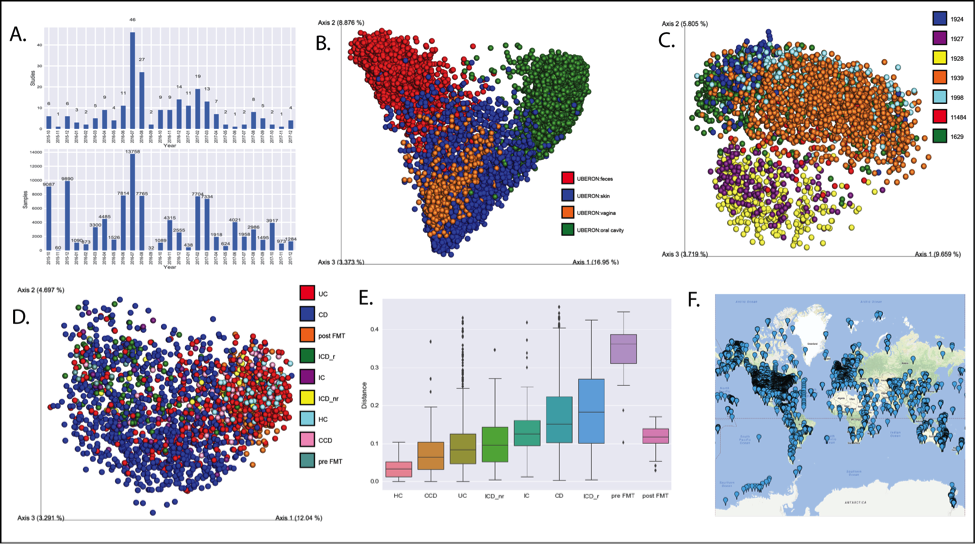
\includegraphics[width=\columnwidth]{chapter_qiita_figures/Figure_1.png}
\caption[Data loaded in Qiita and uploaded to EBI]{\textbf{Data loaded in Qiita and uploaded to EBI.} A. Monthly studies and sample
depositions to EBI-ENA via Qiita. B. Geographical distribution of the samples present in Qiita.}
\label{QiitaF1}
\end{figure}

To exemplify Qiita’s meta-analysis utility, we tested the reproducibility of a
study of how microbiomes of ~\gls{ibd} subtypes relate to those of healthy
individuals~\cite{Halfvarson2017}. We combined the 16S data from three studies
of IBD-affected cohorts ~\cite{Halfvarson2017,Gevers2014} and iHMP, with the HMP1
study of healthy individuals ~\cite{Consortium2012} and another study samples of
Clostridium difficile-affected patients that underwent a Fecal Matter Transplant
(FMT) ~\cite{Weingarden2015}. Using the web interface, we computed Unweighted
UniFrac ~\cite{Lozupone2005} and performed Principal Coordinates Analysis (PCoA).
The plot shows the expected clustering via the body site of the sample (Figure ~\ref{QiitaF2}A).
However, when we examine only fecal samples (‘UBERON:feces’ category), we observe a
pattern explained by sequencing platform as previously observed ~\cite{Lozupone2013}, Figure ~\ref{QiitaF2}B.
Restricting analysis to samples using the same sequencing platform (all but the HMP1 study),
we observe clustering of the different IBD subtypes as previously reported ~\cite{Halfvarson2017,Gevers2014},
Figure ~\ref{QiitaF2}C. Using the feces-only distance matrix generated via the Qiita interface,
we used QIIME2 to calculate the distance from each sample to a “healthy plane”~\cite{Halfvarson2017},
replicating the PCoA result across these independent studies. The samples from the C. difficile
patients are also further from the healthy plane than those from the IBD subtypes,
yet are much closer to the healthy plane after restoration of the microbiome via FMT,
Figure ~\ref{QiitaF2}D. This entire analysis took less than 5 minutes of person-time
to perform, and did not require manual intervention once the processing pipeline
was initiated until the use of the files offline in a Jupyter Notebook ~\footnote{\url{https://github.com/knightlab-analyses/qiita-paper}}.
As this example demonstrates, Qiita is a powerful tool to combine and compare
studies for meta-analyses and represents a significant advance for promoting
facile data analysis within the microbiome research community.

\begin{figure}[htbp]
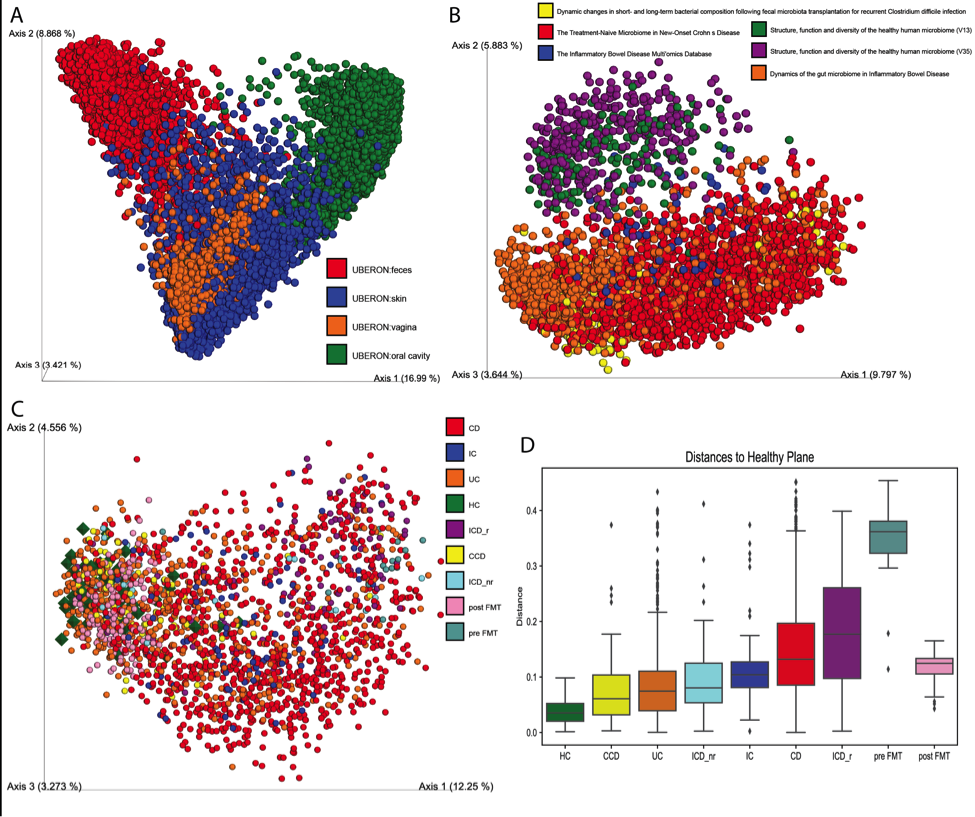
\includegraphics[width=\columnwidth]{chapter_qiita_figures/Figure_2.png}
\caption[Example Meta-Analysis in Qiita]{\textbf{Example Meta-Analysis in Qiita.} A. Unweighted UniFrac PCoA Meta-Analysis
of three studies examining different IBD sub-types, C. difficile patients that underwent
FMT, and the HMP1 and iHMP target gene data, where we can see strong clustering by body habitat.
B. Only fecal samples from the same studies, showing separation due to wet-lab processing;
in purple, yellow and orange HMP1 and iHMP samples. C. Removal of samples with different
processing reproduces the PCoA resembling published results on the distribution of IBD sub-types
(healthy samples as dark green diamonds). D. Calculating distances from a healthy
plane~\cite{Halfvarson2017}, we can reproduce the results (which took several
months to compile and compute originally), and even see how the distances from the
patients with a C. difficile infection have larger distances before FMT and smaller
afterwards.}
\label{QiitaF2}
\end{figure}

By establishing an accessible path from annotated data to consistent and interoperable
results, Qiita provides a practical way to harness the growth of sequence data
for continuing value beyond its initial use by applying the “living data” concept~\cite{Wang2016}
of ongoing reprocessing and annotation. Centralizing data storage and computation
alleviates the substantial burden of independently maintaining compute resources.
The web-based interface for Qiita allows users to avoid operating-system restrictions
and obviates the need to train users to install, configure, and troubleshoot software
via the command-line. To date, this resource hosts over 50TB of omics data from over
460,000 samples originating from studies that span the world, Figure ~\ref{QiitaF1}B.
More than 168,000 of these samples, including the entire recently released ~\gls{emp}~\cite{Thompson2017}
are public and immediately available for meta-analyses. As this collection grows,
it will become increasingly important to improve the quality of associated metadata.
Currently, Qiita requires MIxS-compliant metadata prior to making sequences public,
ensuring that samples available for meta-analysis meet a minimum standard; additionally,
expert-curated “Gold” studies with exceptional metadata are highlighted both as common
references and to promote better practices in the community.

The power of this configuration has already been demonstrated through publications
during the developmental stage of the platform and in our Qiita workshops, carried
out regularly since early 2017 at UC San Diego Center for Microbiome Innovation
\footnote{\url{http://cmi-workshop.readthedocs.io/en/latest/}}. Though not yet
officially released, Qiita has already received over 100 citations in Google Scholar,
and numerous publications have used samples from multiple studies in Qiita to
perform meta-analyses. Additionally, custom instances of Qiita can be easily set
up on virtual or physical machines to host specific datasets, as we have exemplified
for the IBDMDB in the iHMP at http://ihmp.ucsd.edu/.

Qiita thus provides a unique resource allowing researchers to contextualize their data,
perform meta-analyses across hundreds of studies and thousands of samples, and
seamlessly deposit data into standards-compliant databases. Critically, a model
of “easy input, consistent output” assures that time and effort spent analyzing
each new study incrementally and usefully adds to the total resource. Qiita will
thus revolutionize the pace of microbiome analyses and meta-analyses.

\subsection{Online methods}

\subsubsection{Code design and availability}

Qiita is designed using a three layer pattern: storage, logic, and interface.
We describe each layer individually.

The storage layer design is a combination of a PostgreSQL 9.3.17 database and a
structured filesystem. This approach allows Qiita to maintain referential integrity
within and between studies, sample metadata, the analysis pipeline(s), and the
commands executed over the different data types. However, the data volume is such
that it can encumber a relational database, so the data (e.g., sequence files,
contingency tables etc.) are stored in standard formats (e.g FASTA, FASTQ, BIOM).
The database maintains file path locations using indirection to allow files to
reside on any number of filesystems. Additionally, this layer also stores the
covariates (metadata) of each sample split in two main tables: a sample and a
preparation information. The sample information are the covariates pertinent to
the sample, while the preparation is how the sample was processed in the wet-lab
and data generation (target gene sequencing, shotgun, metabolomic, etc).

The Qiita logic layer is written in Python using Object Oriented Programming,
defining an object for each important element of the system. All data in Qiita are
represented by an “artifact” object. An artifact represents a collection of files
which reside on the filesystem, the logical types associated with each file, and a
logical type of the artifact itself. Commands can specify which type of artifacts
they accept as input and which type of artifacts they generate as output. The
type of artifacts and the commands used to analyze artifacts are defined by Qiita
plugins, which encapsulate the compute logic. Qiita defines two types of plugins:
Qiita Type Plugins and Qiita Plugins. The Qiita Type Plugins define new artifact
types, and is how data are imported into Qiita. A Qiita Type Plugin must define
only two operations: “Validate” and “Generate HTML summary”. The “Validate” operation
receives as input the set of files, and user associated types, for a new artifact
and the preparation information and determines if the set of files defines a valid
“artifact” for the given preparation. For example, in the case of a set of per-sample
FASTQ files, the validator checks that each of the samples has a unique file,
and that the names of these files match those in the run\_prefix column in the
preparation information. The “Generate HTML summary” obtains the contents of an
artifact and generates an HTML file summarizing the contents of such artifact.
This summary provides a user-interpretable overview of the artifact, usually
helpful enough to determine if something went wrong with the processing of the
artifact. In contrast, the Qiita Plugin represents a collection of logically
related commands (e.g., methods for constructing distance matrices). Each command
within a Qiita Plugin accepts one or more artifacts as input, runtime parameters,
and produces one or more artifacts as output. Each command execution is logged in
the Qiita relational database, specifically, Qiita stores the plugin used, the
command executed within the plugin, the artifacts provided as inputs, the parameters
specified, and the artifacts generated.

The motivation for a modular plugin system is separation of concerns and
encapsulation as each plugin runs in its own discrete environment and communicates
with Qiita through an internal communication layer. This approach allows the plugins
to be written in any programming language, with plugin specific dependencies, without
introducing dependency conflicts with other plugins in the system. These environments
are managed using plugin-specific conda environments. To facilitate the development
of new Qiita plugins by external developers, we have created a Qiita client
library \footnote{\url{https://github.com/qiita-spots/qiita_client}} and two
Cookiecutter (Qiita Type Plugin \footnote{\url{https://github.com/qiita-spots/qtp-template-cookiecutter}}
and Qiita Plugin \footnote{\url{https://github.com/qiita-spots/qp-template-cookiecutter}})
templates that set up the boilerplate code needed for an initial plugin repository and communication with Qiita.

The interface layer is a web-based interface accessible via Google Chrome, and that
is powered from the server side via Tornado 3.1.1 \footnote{\url{http://www.tornadoweb.org/}}.
The interface design and implementation has gone through multiple rounds of review,
utilizing feedback kindly provided by users attending Qiita workshops.

The source code, and comprehensive test suite, for the Qiita package can be found
in https://github.com/biocore/qiita. The source code for the officially supported
Qiita plugins can be found under the qiita-spots GitHub organization at
https://github.com/qiita-spots. All source code in the qiita repository and
qiita-spots organization are BSD-licensed.

\subsubsection{Data analysis}
One of the most important items for a successful meta-analysis is consistency
during the data processing. To achieve this consistency, Qiita processes all
raw data with one of several standard parameter sets, based on the recommendations
published in the literature. The parameters for demultiplexing and quality control
the 16S rRNA gene sequences are based on the assessment performed Bokulich et al. ~\cite{Bokulich2013},
while the parameters for OTU picking are based on the recommendations provided in
Navas-Molina et al ~\cite{Navas-Molina2013}. In addition to OTU picking,
Qiita also permits sub-OTU sequence clustering with Deblur ~\cite{Amir2017}. In
the deblur manuscript, the authors used more stringent quality control
parameters from those outlined by Bokulich et al. ~\cite{Bokulich2013}.

\subsubsection{Data availability}

All data used is available via Qiita and EBI (where applicable). The Human Microbiome
Project (HMP) and Integrative Human Microbiome Project (iHMP) data is available
via the HMP Data Analysis and Coordination Center (DACC) \footnote{\url{https://hmpdacc.org/}}.
Analytical steps for this paper can be found in \footnote{\url{https://github.com/knightlab-analyses/qiita-paper}}.
Additionally, the Qiita Analysis can be found here \footnote{\url{https://qiita.ucsd.edu/analysis/description/15093/}},
you must be log in to Qiita to access it.
